\documentclass[11pt,a5]{article}
\usepackage[utf8]{inputenx}
\usepackage[spanish]{babel}
\usepackage{graphicx}
\usepackage{wrapfig}
\usepackage[usenames,dvipsnames]{xcolor}
\usepackage{framed}
\usepackage[framemethod=TikZ]{mdframed}
\usepackage{fancybox}
\usepackage{wallpaper}
\usepackage{caption}
\usepackage{subcaption}


% Estilo de página %% NO CAMBIAR!!
\pagestyle{empty} % no page number
\parskip 7.2pt    % space between subsubsection*s
\parindent 0pt   % indent for new subsubsection*
\textwidth 4.5in  % width of text
\columnsep 0.8in  % separation between columns
\usepackage{geometry}
\geometry{left=0.5in,top=0.5in,right=0.5in,bottom=0.5in} %margins

% Colores de la página de osgeo
\definecolor{VerdeClaro1}{RGB}{193,226,165}
\definecolor{VerdeClaro2}{RGB}{160,206,103}
\definecolor{VerdeOscuro1}{RGB}{73,169,66}
\definecolor{VerdeOscuro2}{RGB}{40,151,40}

% Definición del estilo de las cajas
\mdfdefinestyle{Caja}{%
    linecolor=VerdeOscuro2,%black!70!green,
    outerlinewidth=0.1em,
    skipabove=.3\baselineskip,
    skipbelow=.3\baselineskip,
    roundcorner=1em,
    leftmargin=.0005\textwidth,
    rightmargin=.0005\textwidth,
    innertopmargin=3ex,
    innerbottommargin=.5\baselineskip,
    innerrightmargin=1em,
    innerleftmargin=1em,
    backgroundcolor=VerdeClaro1!50!white,
    frametitlerule=true,
    frametitlerulecolor=VerdeOscuro2,%black!70!green,
    frametitlebackgroundcolor=VerdeOscuro1,%green!50!black,
    frametitlerulewidth=0.2em,
    frametitlefont=\sffamily
    }

\mdfdefinestyle{CajaContactos}{%
    linecolor=VerdeOscuro2,%black!70!green,
    outerlinewidth=0.1em,
    skipabove=.4\baselineskip,
    skipbelow=.4\baselineskip,
    roundcorner=1em,
    %leftmargin=.0005\textwidth,
    %rightmargin=.0005\textwidth,
    innertopmargin=1ex,
    innerbottommargin=.5\baselineskip,
    innerrightmargin=1em,
    innerleftmargin=1em,
    backgroundcolor=VerdeClaro1!50!white,
    frametitlerule=true,
    frametitlerulecolor=VerdeOscuro2,
    frametitlebackgroundcolor=VerdeOscuro1,
    frametitlerulewidth=0.2em,
    frametitlefont=\sffamily
    }

% Colores de la página de OSGeo
%\newcommand{\web}{\color{VerdeOscuro2!50!black}\large\center\texttt}
\newcommand{\web}[1]{\texttt{\color{VerdeOscuro2!50!black}\large #1}}
\newcommand{\alert}[1]{\textbf{\color{VerdeOscuro2!80!black}#1}}

%% INICIA EL DOCUMENTO
\begin{document}

% Tipo de fuente Sans-Serif para todo el documento
\sffamily

\begin{figure}[ht]
  \begin{center}
    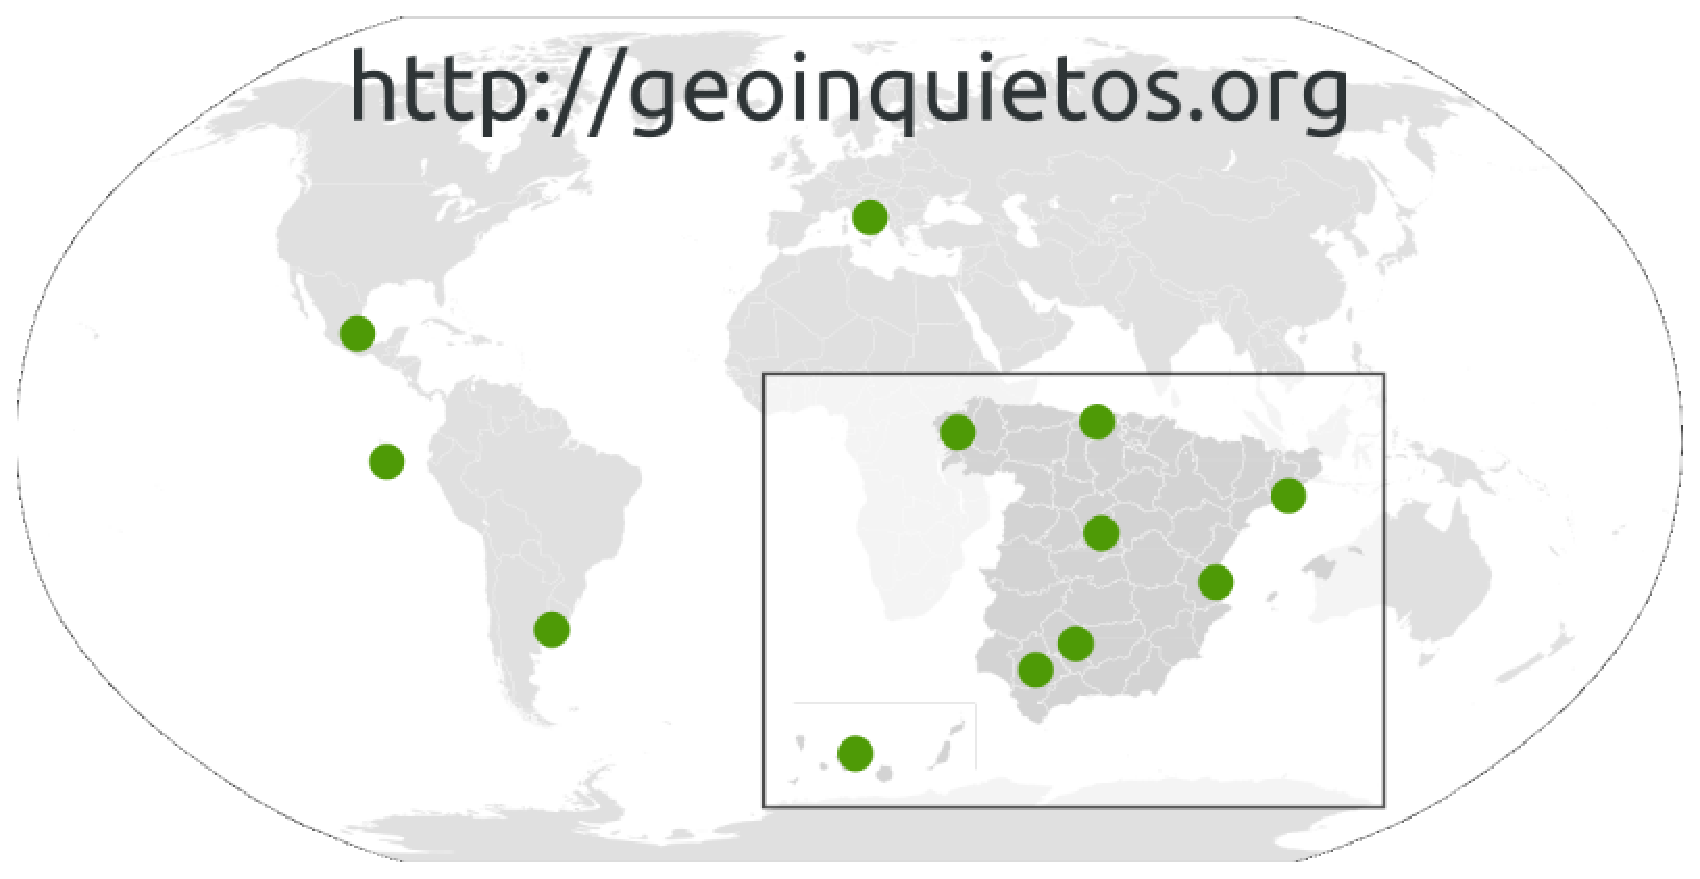
\includegraphics[width=0.65\textwidth]{img/Geoinquietos-world}
  \end{center}
\end{figure}

\alert{Geoinquietos} son encuentros locales informales entre gente que comparte
inquietudes, intereses, experiencias o cualquier idea en el ámbito de la
geomática, el software libre y la tecnología geoespacial (todo aquello
relacionado con el ámbito GEO y SIG). Son reuniones distendidas que suelen
constar de una o varias pequeñas presentaciones o talleres sobre un tema
relacionado con la tecnología y la información geográfica. 

Los Geoinquietos se han extendido ya por Barcelona, Cantabria, Córdoba, Madrid,
Tenerife, Valencia y la zona Norte. También se han creado grupos de geoinquietos
en Buenos Aires, Roma y las Islas Galápagos.

Los participantes y asistentes toman un papel participativo y activo generando
un ambiente donde fluyen ideas y experiencias en torno a la tecnología y la
innovación. \alert{Cualquier persona está invitada} a asistir a las actividades
de Geoinquietos, con el único requisito de querer \alert{compartir}
conocimientos y \alert{aprender} de los demás.

El Portal Geoinquietos (\alert{\texttt{http://geoinquietos.drupalgardens.com/}})
centraliza toda la información sobre los diferentes grupos locales. También
puedes buscar y utilizar el hashtag \alert{\#geoinquietos} en Twitter. 

%\begin{figure}[h]
%  \begin{center}
%    
\includegraphics[width=0.10\textwidth]{img/logo_geoinquietosmad}
%  \end{center}
%\end{figure}

\begin{figure}[h]
        \centering
        \begin{subfigure}[b]{0.12\textwidth}
                \centering
                
\includegraphics[width=\textwidth]{img/logo_geoinquiets}
        \end{subfigure}%
        ~
        \begin{subfigure}[b]{0.12\textwidth}
                \centering
                
\includegraphics[width=\textwidth]{img/logo_geoinquietosbas}
        \end{subfigure}%
        ~
        \begin{subfigure}[b]{0.12\textwidth}
                \centering
                
\includegraphics[width=\textwidth]{img/logo_geoinquietoscan}
        \end{subfigure}%
        ~
        \begin{subfigure}[b]{0.12\textwidth}
                \centering
                
\includegraphics[width=\textwidth]{img/logo_geoinquietosmad}
        \end{subfigure}%
        ~
        \begin{subfigure}[b]{0.12\textwidth}
                \centering
                
\includegraphics[width=\textwidth]{img/logo_geoinquietosten}
        \end{subfigure}%
        ~
        \begin{subfigure}[b]{0.12\textwidth}
                \centering
                \includegraphics[width=\textwidth]{img/logo_geoinquietosval}
        \end{subfigure}%
        ~
        \begin{subfigure}[b]{0.12\textwidth}
                \centering
                
\includegraphics[width=\textwidth]{img/logo_xeoinquedos}
        \end{subfigure}%
\end{figure}

\begin{center}
\color{VerdeOscuro2!50!black}\huge Geoinquietos Madrid
\end{center}

\alert{Geoinquietos Madrid} surge como iniciativa para ponernos en contacto en
la zona de Madrid. Se trata de un evento donde compartir inquietudes, intereses,
experiencias o cualquier idea, que se relacione con el ambito geomático.

\begin{center}
\begin{minipage}{0.3\textwidth}
  \begin{center} \large
    \begin{mdframed}[style=CajaContactos, frametitle={\Large\color{green!10!white} Twitter}]
      \web{@geoinquietosmad}
    \end{mdframed}
  \end{center}
\end{minipage}
%
\begin{minipage}{0.65\textwidth}
  \begin{center} \large
    \begin{mdframed}[style=CajaContactos, frametitle={\Large\color{green!10!white} Lista de correo}]
      \web{http://lists.osgeo.org/mailman/listinfo/madrid}
    \end{mdframed}
  \end{center}
\end{minipage}

\begin{minipage}{0.9\textwidth}
\begin{center} \large
    \begin{mdframed}[style=CajaContactos, frametitle={\Large\color{green!10!white} Wiki}]
      \web{http://wiki.osgeo.org/wiki/Capítulo\_Local\_de\_la\_comunidad\_hispanohablante}
    \end{mdframed}
  \end{center}
\end{minipage}
\end{center}

\newpage


\mdfsetup{frametitlealignment=\center}

\begin{center}
\color{VerdeOscuro2!50!black}\Huge Minimanual de OpenStreetMaps
\end{center}

\begin{mdframed}[style=Caja, frametitle={\Large\color{green!10!white}Portal OpenStreetMap}]
     Acceder al portal de OpenStreetMap (OSM), visualizar el mapa,
    acceder al WIKI y al blog... 

    \web{http://www.openstreetmap.org}
\end{mdframed}

\begin{mdframed}[style=Caja, frametitle={\Large\color{green!10!white}Sección española de OpenStreetMap}]
Acceder al portal de la sección española de OpenStreetMap (OSM), visualizar el
mapa, acceder al WIKI y al blog...

\web{http://www.openstreetmap.es}
\end{mdframed}

\begin{mdframed}[style=Caja, frametitle={\Large\color{green!10!white}Ver un mapa}]
 Si conocemos las coordenadas Longitud y Latitud del centro del mapa, y añadimos
un nivel de zoom entre 0 y 18 podemos crear un enlace al mapa personalizado.

\web{http://www.openstreetmap.org?lon=-3.83\&lat=43.47\&zoom=13}
\end{mdframed}

\begin{mdframed}[style=Caja, frametitle={\Large\color{green!10!white}Distintos Renders}]
 Si añadimos un parametro \alert{layers} podemos seleccionar entre Mapnik (M),
Osmarender (O) y CycleMap (C).

\web{http://www.openstreetmap.org?lon=-3.83\&lat=43.47\&zoom=13\&layers=C}
\end{mdframed}

\begin{mdframed}[style=Caja, frametitle={\Large\color{green!10!white}Marcadores}]
 Añadiendo una pareja de parámetros \alert{mlon} y \alert{mlat} podemos añadir un marcador
en las coordenadas deseadas.

\web{http://www.openstreetmap.org?mlon=-3.83\&mlat=43.47\&zoom=13\&layers=O}
\end{mdframed}

\begin{mdframed}[style=Caja, frametitle={\Large\color{green!10!white}OpenSeaMap}]
 También se está trabajando en cartas naúticas.

\web{http://www.openseamap.org}
\end{mdframed}

\begin{mdframed}[style=Caja, frametitle={\Large\color{green!10!white}OpenTouchMap}]
 Esta versión funciona en las pantallas táctiles de los móviles.

\web{http://www.opentouchmap.org?lon=-3.76\&lat=40.385\&zoom=15}
\end{mdframed}

\end{document}
